\graphicspath{ {Figures/TMethod/Main/} {Figures/TMethod/ResidualsFFT/} {Figures/TMethod/Comparison/} {Figures/TMethod/RandomSeeds/} }

\chapter{T Method Fit}
\label{Ch:TMethod}

This entire chapter is a work in progress.


While not the main focus of my analysis, I also perform a T method fit to the data along with the ratio fit. This is useful as a comparison to the ratio method results, and can also provide useful parameter information that the ratio method has trouble getting at. I do not perform systematic studies, and only perform analysis checks like fit start time scans to verify that the T method fit is working correctly. In my T method fit, I include all CBO terms, the vertical waist, and lost muons, as described in Chapter \ref{Ch:Procedures}. The same fit start and end times as used in the ratio fit of ($\SI{30}{\mu s} - \SI{650}{\mu s}$) are used here as well.

The results for a T-Method fit are shown in Figure \ref{fig:TMethod_moduloPlot}, with a table of the results with parameter information shown in Table \ref{Tab:FitParamsTMethod}. The correlation matrix for the T-Method fit is shown in Table \ref{Tab:CorrMatTMethod}.

An FFT of the results is included for posterity in Figures 



A comparison between the ratio and T-Method results are shown in Table

There is a slight difference in data that is fitted between the T method and the ratio method. Because of the time shifting that is done in the ratio method, there is a quarter \gmtwo periods worth of data starting at $\SI{30}{\mu s}$ that is replaced by data before $\SI{30}{\mu s}$. This shouldn't change much but should be kept in mind when comparing...



	\begin{figure}[]
		\centering
		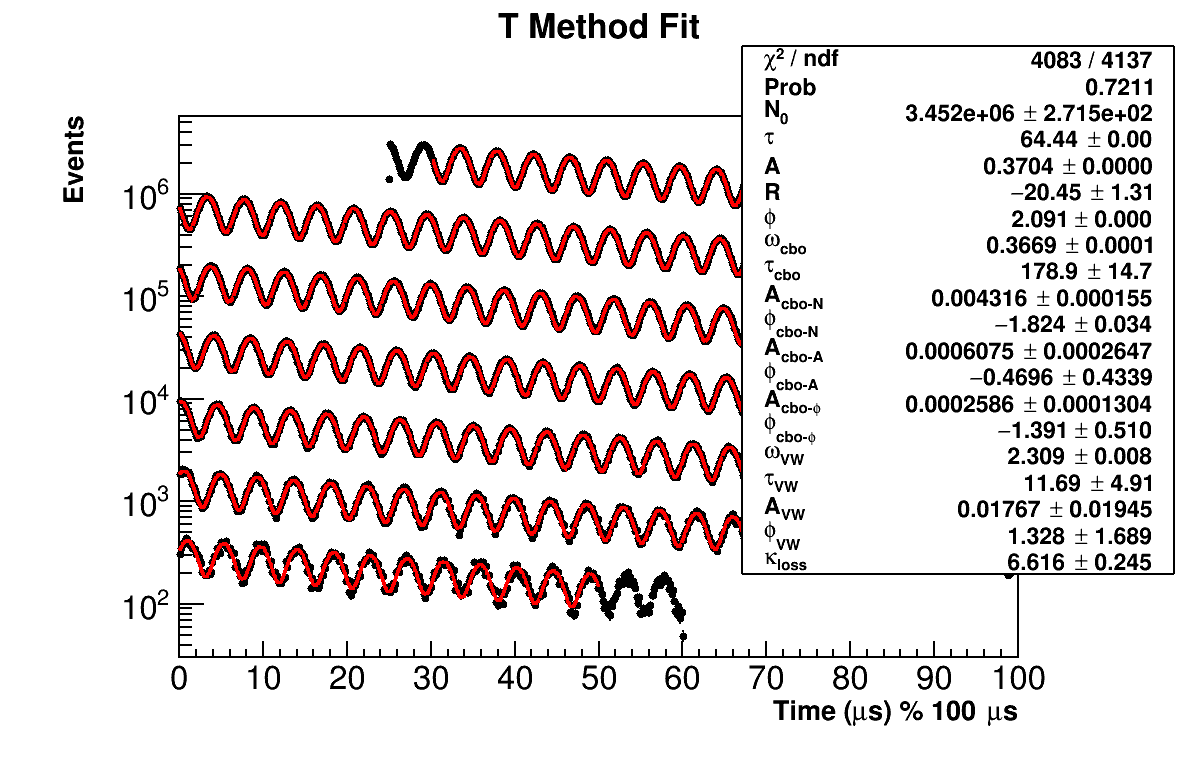
\includegraphics[width=\textwidth]{TMethod_moduloPlot}
	    \caption[TMethod_moduloPlot]{Final fit result for the 60 hour dataset for a T method fit. The x axis is in units of $\mu$s modulo 100 $\mu$s, with successive portions of the data points and fit shifted downwards on the plot. R is blinded locally. The fit ranges from 30 $\mu$s to 650 $\mu$s.}
	    \label{fig:TMethod_moduloPlot}
	\end{figure}

	\begin{table}[]
	\centering
	\setlength\tabcolsep{10pt}
	\renewcommand{\arraystretch}{1.2}
	\begin{tabular*}{.8\linewidth}{@{\extracolsep{\fill}}|l|l|c|c|}
	  \hline
	  	\multicolumn{4}{|c|}{\textbf{T-Method Fit Results}} \\
	  \hline\hline
	  	\multicolumn{2}{|c}{$\chi^{2}$/NDF}       				&  \multicolumn{2}{c|}{$2964/3137$}  \\
	  	\multicolumn{2}{|c}{P value}         	 				&  \multicolumn{2}{c|}{$0.9867$}  \\
	  \hline\hline
	  	Parameter & Descriptor & Value & Error \\
	  \hline
		$N_{0}$    			  & Number  	    			&  $\SI{3.327e6}{}$  	&	$\SI{2.668e2}{}$  \\
		$\tau$    			  & Muon Lifetime $(\mu s)$ 	&  $64.44$  			&	$\SI{3.965e-3}{}$  \\
		$A$    			 	  & Asymmetry  	    			&  $0.3704$  			&	$\SI{4.493e-5}{}$  \\
		$R$     			  & R (ppm, blinded)   	 		&  $-19.88$  			&	$1.373$  \\
		$\phi$   			  & \gmtwo Phase         		&  $2.091$  			&	$\SI{2.249e-4}{}$  \\
		$\omega_{cbo}$   	  & CBO Frequency $(MHz)$       &  $0.37$  				&	$\SI{}{}$  \\
		$\tau_{cbo}$          & CBO Lifetime $(\mu s)$ 	    &  $182.1$  			&	$15.67$  \\
		$A_{cbo-N}$   	 	  & CBO N Amplitude      		&  $0.00449$  			&	$\SI{2.365e-4}{}$  \\
		$\phi_{cbo-N}$   	  & CBO N Phase       	 		&  $-1.835$  			&	$0.1017$  \\
		$A_{cbo-A}$   	 	  & CBO A Amplitude      		&  $0.00449$  			&	$\SI{2.365e-4}{}$  \\
		$\phi_{cbo-A}$   	  & CBO A Phase       	 		&  $-1.835$  			&	$0.1017$  \\
		$A_{cbo-\phi}$   	  & CBO $\phi$ Amplitude      	&  $0.00449$  			&	$\SI{2.365e-4}{}$  \\
		$\phi_{cbo-\phi}$     & CBO $\phi$ Phase       	 	&  $-1.835$  			&	$0.1017$  \\
		$\omega_{VW}$   	  & VW Frequency $(MHz)$        &  $2.3$  				&	$\SI{}{}$  \\
		$\tau_{VW}$           & VW Lifetime $(\mu s)$ 	    &  $18$  				&	$15.67$  \\
		$A_{cbo-VW}$   	 	  & VW Amplitude      			&  $0.001$  			&	$\SI{2.365e-4}{}$  \\
		$\phi_{cbo-VW}$   	  & VW Phase       	 			&  $-0.34$  			&	$0.1017$  \\
		$\kappa_{loss}$   	  & Lost Muon Normalization     &  $6.7$  			    &	$2$  \\
	  \hline
	\end{tabular*}
	\caption{Table of T-Method fit results.}
	\label{Tab:FitParamsTMethod}
	\end{table}

\begin{landscape}
	\begin{table}[]
	% \resizebox{!}{\columnheight}{%
	% \scalebox{0.5}{%
	\setlength\tabcolsep{0pt}
	\scalebox{0.7}{%
	\begin{tabular*}{1.5\linewidth}{@{\extracolsep{\fill}}lLBLLLLLLLLLLLLLLLLLL}
	  \toprule
	            & \thead{$N_{0}$} & \thead{$\tau$} & \thead{$A$} & \thead{$R$} & \thead{$\phi$} & \thead{$\omega_{cbo}$} & \thead{$\tau_{cbo}$} & \thead{$A_{cbo-N}$} & \thead{$\phi_{cbo-N}$} & \thead{$A_{cbo-2N}$} & \thead{$\phi_{cbo-2N}$} & \thead{$A_{cbo-A}$} & \thead{$\phi_{cbo-A}$} & \thead{$A_{cbo-\phi}$} & \thead{$\phi_{cbo-\phi}$} & \thead{$\omega_{VW}$} & \thead{$\tau_{VW}$} & \thead{$A_{VW}$} & \thead{$\phi_{VW}$} & \thead{$\kappa_{loss}$} \\
	  \midrule
		$N_{0}$    			 &  1.0000  &  0.0049  & -0.0068  & -0.0166  &  0.0000  & -0.0098  &  0.0233 &  1.0000  &  0.0049  & -0.0068  & -0.0166  &  0.0000  & -0.0098  &  0.0233  &  0.0049  & -0.0068  & -0.0166  &  0.0000  & -0.0098  &  0.0233  \\
		$\tau$    			 &  1.0000  &  0.0049  & -0.0068  & -0.0166  &  0.0000  & -0.0098  &  0.0233 &  1.0000  &  0.0049  & -0.0068  & -0.0166  &  0.0000  & -0.0098  &  0.0233  &  0.0049  & -0.0068  & -0.0166  &  0.0000  & -0.0098  &  0.0233  \\
		$A$    			 	 &  1.0000  &  0.0049  & -0.0068  & -0.0166  &  0.0000  & -0.0098  &  0.0233 &  1.0000  &  0.0049  & -0.0068  & -0.0166  &  0.0000  & -0.0098  &  0.0233  &  0.0049  & -0.0068  & -0.0166  &  0.0000  & -0.0098  &  0.0233  \\
		$R$     			 &  0.0049  &  1.0000  & -0.8300  & -0.0204  &  0.0000  &  0.0207  &  0.0282 &  1.0000  &  0.0049  & -0.0068  & -0.0166  &  0.0000  & -0.0098  &  0.0233  &  0.0049  & -0.0068  & -0.0166  &  0.0000  & -0.0098  &  0.0233  \\
		$\phi$   			 & -0.0068  & -0.8300  &  1.0000  &  0.0280  &  0.0000  & -0.0287  & -0.0387 &  1.0000  &  0.0049  & -0.0068  & -0.0166  &  0.0000  & -0.0098  &  0.0233  &  0.0049  & -0.0068  & -0.0166  &  0.0000  & -0.0098  &  0.0233  \\
		$\omega_{cbo}$   	 & -0.0166  & -0.0204  &  0.0280  &  1.0000  &  0.0000  &  0.0773  & -0.8585 &  1.0000  &  0.0049  & -0.0068  & -0.0166  &  0.0000  & -0.0098  &  0.0233  &  0.0049  & -0.0068  & -0.0166  &  0.0000  & -0.0098  &  0.0233  \\
		$\tau_{cbo}$		 &  0.0000  &  0.0000  &  0.0000  &  0.0000  &  1.0000  &  0.0000  &  0.0000 &  1.0000  &  0.0049  & -0.0068  & -0.0166  &  0.0000  & -0.0098  &  0.0233  &  0.0049  & -0.0068  & -0.0166  &  0.0000  & -0.0098  &  0.0233  \\
		$A_{cbo-N}$   	 	 & -0.0098  &  0.0207  & -0.0287  &  0.0773  &  0.0000  &  1.0000  & -0.0656 &  1.0000  &  0.0049  & -0.0068  & -0.0166  &  0.0000  & -0.0098  &  0.0233  &  0.0049  & -0.0068  & -0.0166  &  0.0000  & -0.0098  &  0.0233  \\
		$\phi_{cbo-N}$   	 &  0.0233  &  0.0282  & -0.0387  & -0.8585  &  0.0000  & -0.0656  &  1.0000 &  1.0000  &  0.0049  & -0.0068  & -0.0166  &  0.0000  & -0.0098  &  0.0233  &  0.0049  & -0.0068  & -0.0166  &  0.0000  & -0.0098  &  0.0233  \\
		$A_{cbo-2N}$   	 	 & -0.0098  &  0.0207  & -0.0287  &  0.0773  &  0.0000  &  1.0000  & -0.0656 &  1.0000  &  0.0049  & -0.0068  & -0.0166  &  0.0000  & -0.0098  &  0.0233  &  0.0049  & -0.0068  & -0.0166  &  0.0000  & -0.0098  &  0.0233  \\
		$\phi_{cbo-2N}$   	 &  0.0233  &  0.0282  & -0.0387  & -0.8585  &  0.0000  & -0.0656  &  1.0000 &  1.0000  &  0.0049  & -0.0068  & -0.0166  &  0.0000  & -0.0098  &  0.0233  &  0.0049  & -0.0068  & -0.0166  &  0.0000  & -0.0098  &  0.0233  \\
		$A_{cbo-A}$   	 	 & -0.0098  &  0.0207  & -0.0287  &  0.0773  &  0.0000  &  1.0000  & -0.0656 &  1.0000  &  0.0049  & -0.0068  & -0.0166  &  0.0000  & -0.0098  &  0.0233  &  0.0049  & -0.0068  & -0.0166  &  0.0000  & -0.0098  &  0.0233  \\
		$\phi_{cbo-A}$   	 &  0.0233  &  0.0282  & -0.0387  & -0.8585  &  0.0000  & -0.0656  &  1.0000 &  1.0000  &  0.0049  & -0.0068  & -0.0166  &  0.0000  & -0.0098  &  0.0233  &  0.0049  & -0.0068  & -0.0166  &  0.0000  & -0.0098  &  0.0233  \\
		$A_{cbo-\phi}$   	 & -0.0098  &  0.0207  & -0.0287  &  0.0773  &  0.0000  &  1.0000  & -0.0656 &  1.0000  &  0.0049  & -0.0068  & -0.0166  &  0.0000  & -0.0098  &  0.0233  &  0.0049  & -0.0068  & -0.0166  &  0.0000  & -0.0098  &  0.0233  \\
		$\phi_{cbo-\phi}$    &  0.0233  &  0.0282  & -0.0387  & -0.8585  &  0.0000  & -0.0656  &  1.0000 &  1.0000  &  0.0049  & -0.0068  & -0.0166  &  0.0000  & -0.0098  &  0.0233  &  0.0049  & -0.0068  & -0.0166  &  0.0000  & -0.0098  &  0.0233  \\
		$\omega_{VW}$   	 & -0.0166  & -0.0204  &  0.0280  &  1.0000  &  0.0000  &  0.0773  & -0.8585 &  1.0000  &  0.0049  & -0.0068  & -0.0166  &  0.0000  & -0.0098  &  0.0233  &  0.0049  & -0.0068  & -0.0166  &  0.0000  & -0.0098  &  0.0233  \\
		$\tau_{VW}$		 	 &  0.0000  &  0.0000  &  0.0000  &  0.0000  &  1.0000  &  0.0000  &  0.0000 &  1.0000  &  0.0049  & -0.0068  & -0.0166  &  0.0000  & -0.0098  &  0.0233  &  0.0049  & -0.0068  & -0.0166  &  0.0000  & -0.0098  &  0.0233  \\
		$A_{VW}$   	 	 	 & -0.0098  &  0.0207  & -0.0287  &  0.0773  &  0.0000  &  1.0000  & -0.0656 &  1.0000  &  0.0049  & -0.0068  & -0.0166  &  0.0000  & -0.0098  &  0.0233  &  0.0049  & -0.0068  & -0.0166  &  0.0000  & -0.0098  &  0.0233  \\
		$\phi_{VW}$   	 	 &  0.0233  &  0.0282  & -0.0387  & -0.8585  &  0.0000  & -0.0656  &  1.0000 &  1.0000  &  0.0049  & -0.0068  & -0.0166  &  0.0000  & -0.0098  &  0.0233  &  0.0049  & -0.0068  & -0.0166  &  0.0000  & -0.0098  &  0.0233  \\
		$\kappa_{loss}$   	 &  0.0233  &  0.0282  & -0.0387  & -0.8585  &  0.0000  & -0.0656  &  1.0000 &  1.0000  &  0.0049  & -0.0068  & -0.0166  &  0.0000  & -0.0098  &  0.0233  &  0.0049  & -0.0068  & -0.0166  &  0.0000  & -0.0098  &  0.0233  \\
	  \bottomrule
	\end{tabular*}}
	\caption{Correlation matrix for the T method fit. The only significant correlation to R is the \gmtwo phase.}
	\label{Tab:CorrMatTMethod}
	% } % resize box
	\end{table}
\end{landscape}

% 1 0.165054 0.020449 -0.043894 0.0460814 0.0251477 -0.0713088 0.0746406 -0.0120761 0.000448665 -0.0231571 0.0276081 0.0258435 -0.0433282 -0.0125253 -0.116929 -0.491199 0.511525 0.120798 0.580002
% 0.165054 1 0.013115 -0.0081023 0.00718629 0.00397994 -0.0249367 0.0279856 0.00363996 -0.0165722 -0.0189651 0.0143383 0.0184532 -0.0332119 -0.00228916 -0.030049 -0.0582218 0.0553853 0.0315517 0.85587
% 0.020449 0.013115 1 0.00457271 -0.00643419 -0.0120546 0.00183131 -0.00441358 0.0190641 -0.0108646 -0.00111318 0.01703 -0.0332041 0.00722317 0.0244077 -0.00819908 -0.0164494 0.0159001 0.00797104 0.0193439
% -0.043894 -0.0081023 0.00457271 1 -0.825871 -0.013326 -0.0251207 0.0301418 0.0176667 0.00926808 -0.00397417 -0.024243 -0.0188661 0.0132179 -0.0139492 0.00123097 -0.0315804 0.0325186 -0.001682 -0.0272026
% 0.0460814 0.00718629 -0.00643419 -0.825871 1 0.0203928 0.0305387 -0.0379982 -0.0262186 -0.0126953 0.0015553 0.0315993 0.0238388 -0.0218659 0.0187872 -0.0105152 0.0324318 -0.0337591 0.0112865 0.0278186
% 0.0251477 0.00397994 -0.0120546 -0.013326 0.0203928 1 0.0293156 -0.0290822 -0.859266 0.00407579 -0.126358 -0.00860036 -0.0382414 -0.0107385 -0.0676264 0.0415026 0.0460602 -0.0458634 -0.0426964 0.0167356
% -0.0713088 -0.0249367 0.00183131 -0.0251207 0.0305387 0.0293156 1 -0.882672 -0.0277876 -0.0112729 0.0103132 -0.0631247 0.0350963 -0.026036 0.00703832 -0.0443646 -0.0334781 0.0329381 0.0462585 -0.0532742
% 0.0746406 0.0279856 -0.00441358 0.0301418 -0.0379982 -0.0290822 -0.882672 1 0.0272893 0.0127065 -0.0116176 0.0588683 -0.0468328 0.0222228 -0.00787962 0.0504634 0.0288027 -0.0277961 -0.0529398 0.0569829
% -0.0120761 0.00363996 0.0190641 0.0176667 -0.0262186 -0.859266 -0.0277876 0.0272893 1 0.00552642 0.115778 0.0168894 0.0314304 0.0146214 0.0647802 -0.0402946 -0.0525064 0.0538094 0.041731 -0.00501849
% 0.000448665 -0.0165722 -0.0108646 0.00926808 -0.0126953 0.00407579 -0.0112729 0.0127065 0.00552642 1 -0.00970564 0.00491864 0.000361061 -0.0284008 -0.0188071 0.0019806 0.00148571 0.00354266 0.000393678 -0.0124258
% -0.0231571 -0.0189651 -0.00111318 -0.00397417 0.0015553 -0.126358 0.0103132 -0.0116176 0.115778 -0.00970564 1 0.0106544 0.0279755 0.0198632 0.00393464 -0.0255058 0.012002 -0.0190534 0.0245884 -0.0250201
% 0.0276081 0.0143383 0.01703 -0.024243 0.0315993 -0.00860036 -0.0631247 0.0588683 0.0168894 0.00491864 0.0106544 1 -0.00792014 0.0056861 -0.00358834 -0.0104079 -0.0128044 0.0133101 0.0103544 0.0234205
% 0.0258435 0.0184532 -0.0332041 -0.0188661 0.0238388 -0.0382414 0.0350963 -0.0468328 0.0314304 0.000361061 0.0279755 -0.00792014 1 0.0353129 0.00258113 0.000498675 -0.0152257 0.016901 0.00133716 0.0247163
% -0.0433282 -0.0332119 0.00722317 0.0132179 -0.0218659 -0.0107385 -0.026036 0.0222228 0.0146214 -0.0284008 0.0198632 0.0056861 0.0353129 1 -0.0143978 -0.001379 0.0458929 -0.0492711 0.00224833 -0.044928
% -0.0125253 -0.00228916 0.0244077 -0.0139492 0.0187872 -0.0676264 0.00703832 -0.00787962 0.0647802 -0.0188071 0.00393464 -0.00358834 0.00258113 -0.0143978 1 0.0232057 -0.00596585 0.0061812 -0.0245489 -0.0078532
% -0.116929 -0.030049 -0.00819908 0.00123097 -0.0105152 0.0415026 -0.0443646 0.0504634 -0.0402946 0.0019806 -0.0255058 -0.0104079 0.000498675 -0.001379 0.0232057 1 -0.678774 0.670825 -0.987439 -0.0805513
% -0.491199 -0.0582218 -0.0164494 -0.0315804 0.0324318 0.0460602 -0.0334781 0.0288027 -0.0525064 0.00148571 0.012002 -0.0128044 -0.0152257 0.0458929 -0.00596585 -0.678774 1 -0.964139 0.675769 -0.289003
% 0.511525 0.0553853 0.0159001 0.0325186 -0.0337591 -0.0458634 0.0329381 -0.0277961 0.0538094 0.00354266 -0.0190534 0.0133101 0.016901 -0.0492711 0.0061812 0.670825 -0.964139 1 -0.667907 0.297175
% 0.120798 0.0315517 0.00797104 -0.001682 0.0112865 -0.0426964 0.0462585 -0.0529398 0.041731 0.000393678 0.0245884 0.0103544 0.00133716 0.00224833 -0.0245489 -0.987439 0.675769 -0.667907 1 0.0836521
% 0.580002 0.85587 0.0193439 -0.0272026 0.0278186 0.0167356 -0.0532742 0.0569829 -0.00501849 -0.0124258 -0.0250201 0.0234205 0.0247163 -0.044928 -0.0078532 -0.0805513 -0.289003 0.297175 0.0836521 1








	\begin{figure}[h]
	\centering
	    \begin{subfigure}[]{0.45\textwidth}
		    \centering
			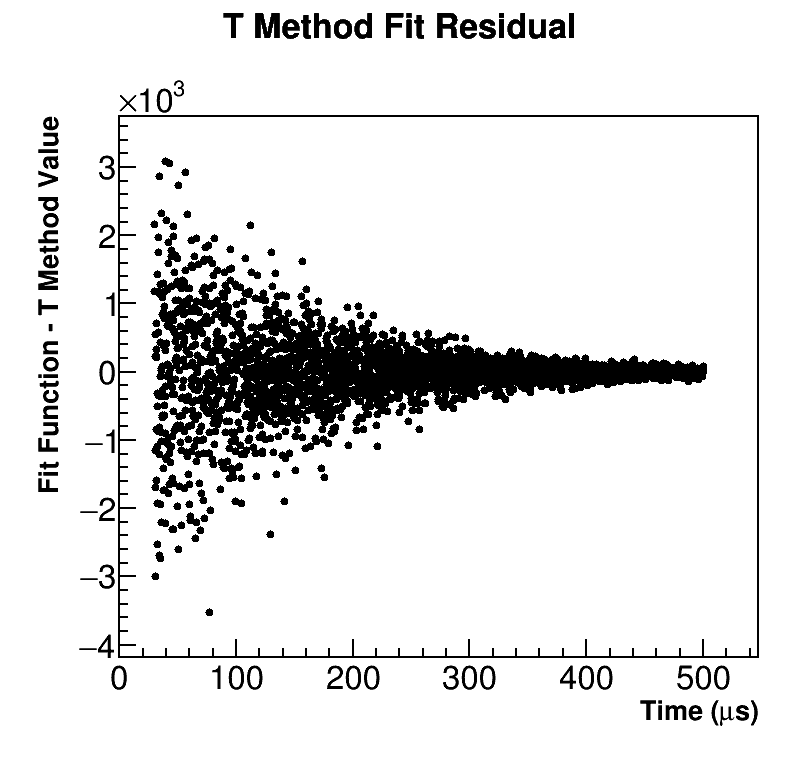
\includegraphics[width=\textwidth]{fitResidual_TMethod}
		    \caption{Fit residuals.}
	    \end{subfigure}
	    \begin{subfigure}[]{0.45\textwidth}
		    \centering
			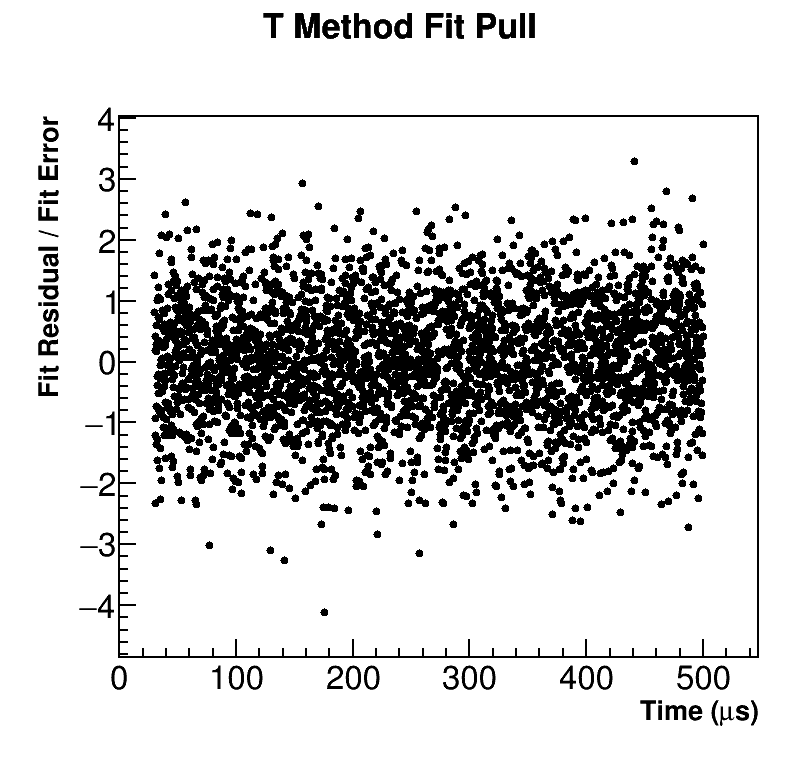
\includegraphics[width=\textwidth]{fitPull_TMethod}
		    \caption{Fit pulls.}
	    \end{subfigure}% %you need this % here to add spacing between subfigures
	    \vspace{4mm}
	    \begin{subfigure}[]{0.7\textwidth}
		    \centering
			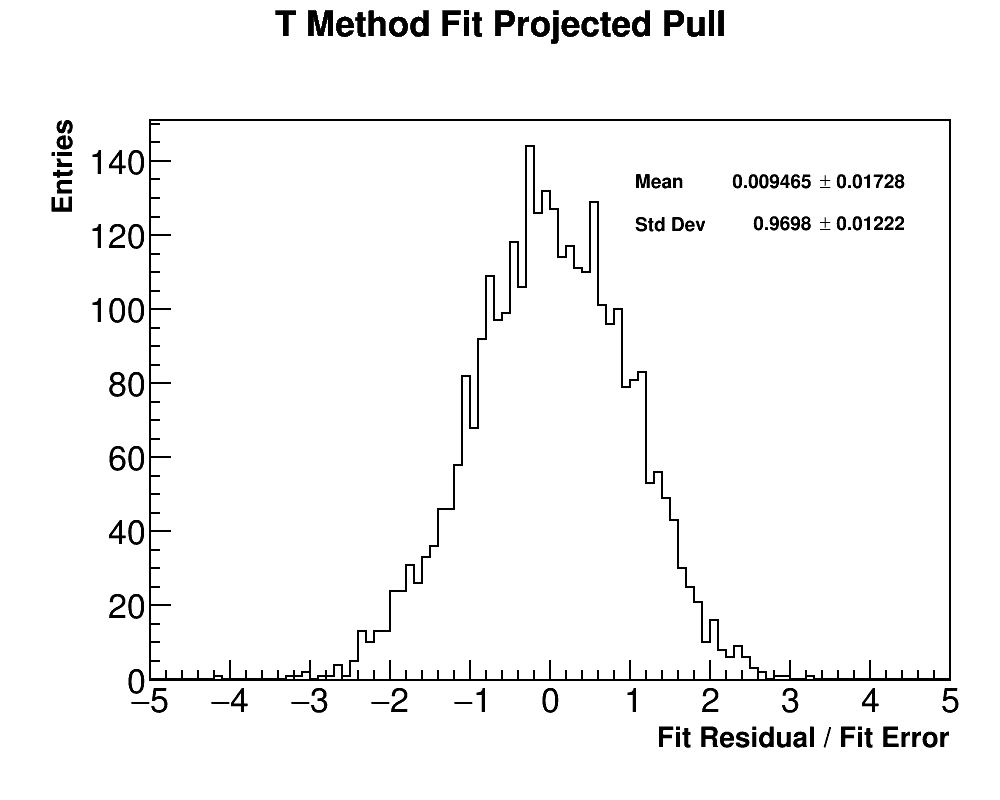
\includegraphics[width=\textwidth]{fitPull_projected_TMethod}
		    \caption{Fit pulls projected onto the y axis. Note the Gaussian shape centered around 0 with unit width.}
	    \end{subfigure}
	\caption[fitResidual_TMethod]{Residuals and pulls for the T Method fit.}
	\label{fig:fitResidual_TMethod}
	\end{figure}

	\begin{figure}[]
		\centering
		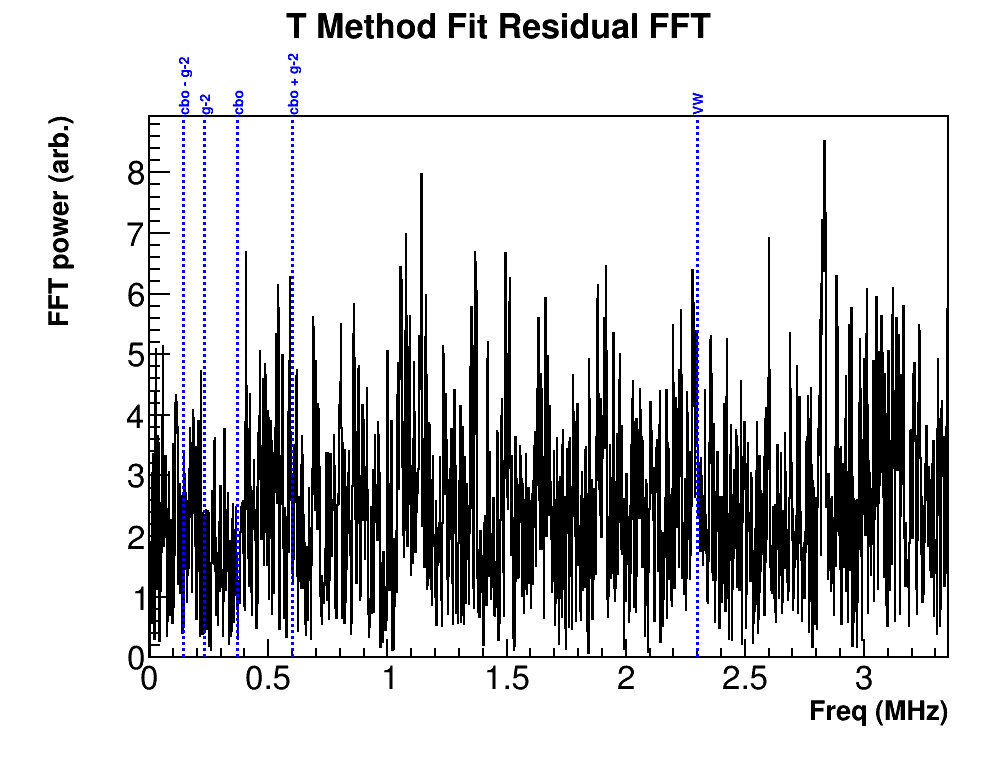
\includegraphics[width=\textwidth]{FFT_TMethodFit}
	    \caption[FFT_TMethodFit]{FFT of the residuals of the T Method fit. No significant peaks remain in the fit residuals after fitting with all terms. Overlayed are dotted lines for the \gmtwo, CBO, and vertical waist frequencies.}
	    \label{fig:FFT_TMethodFit}
	\end{figure}

	\begin{figure}[]
		\centering
		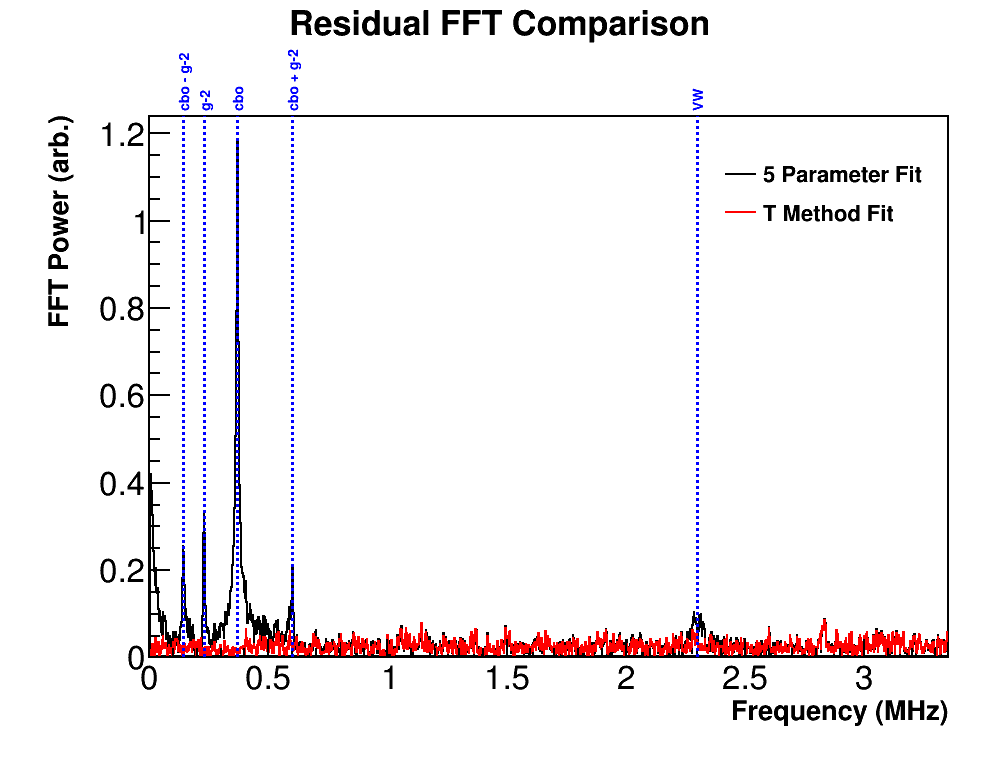
\includegraphics[width=\textwidth]{FFTComparison_TMethod}
	    \caption[FFTComparison_TMethod]{A plot of the FFT of the residuals of the fit for the five parameter fit compared to the T Method fit. In black is the FFT for a five parameter fit, where peaks for the CBO and vertical waist can be seen as well as the \gmtwo peak. In red is the FFT of the T Method fit residuals.}
	    \label{fig:FFTComparison_TMethod}
	\end{figure}

\clearpage

	T method fits were performed for 20 random sees as was done for the ratio method fit. The results are shown in Figure \ref{Subfig:RVsRandomSeedTMethod}. Results are consistent with each other as they should be. The average R value for the T method fits is -19.82 ppm.

	\begin{figure}[]
	\centering
	    \begin{subfigure}[t]{0.45\textwidth}
		    \centering
			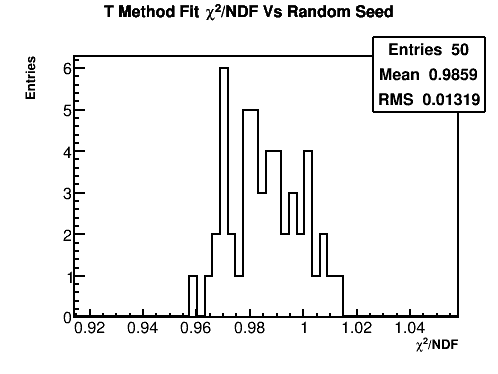
\includegraphics[width=\textwidth]{TMethod_Chi2NDF_Vs_Iter_Canv_hist}
		    \caption{$\chi^{2}$/NDF values for 20 random seeds.}
	    \end{subfigure}
	    \begin{subfigure}[t]{0.45\textwidth}
		    \centering
			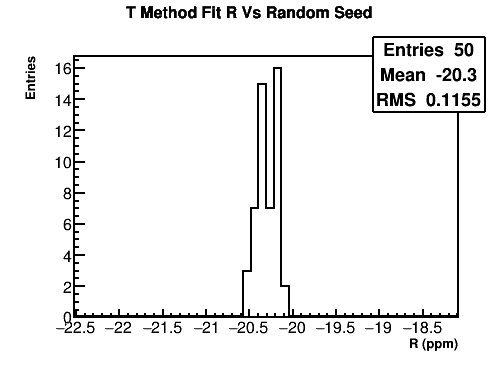
\includegraphics[width=\textwidth]{TMethod_R_Vs_Iter_Canv_hist.png}
		    \caption{R values for 20 random seeds.}
		\label{Subfig:RVsRandomSeedTMethod}
	    \end{subfigure}% %you need this % here to add spacing between subfigures
	\caption[RandomSeedsTMethod]{Plotted is the $\chi^{2}$/NDF and fitted R value for 20 random seeds for the T method fit.}
	\label{fig:RandomSeedsTMethod}
	\end{figure}

\clearpage

\section{Toy MC Comparison}


In order to assist in combining the ratio method results with those of the other analyzers and their T method results, it's useful to perform an MC comparison between the ratio and T method fits. To do this I generated 100 pseudo-experiments in MC. Each pseudo-experiment consisted of a single set of ``positron'' data, generated using a 1D \texttt{ROOT} function corresponding to an energy threshold time histogram. The amount of stats in each pseudo-experiment was chosen to be comparable to the 60H dataset. This single set of hits was then randomized with 50 different random seeds, where the times of the generated hits were randomized in the same way as was done for data to remove the fast rotation. The times were also randomly split into the separate U and V histograms to form the ratio. In this way each pseudo-experiment corresponds to an idealized approximation of the 60H dataset, with 50 different random seeds applied before fitting.

5 parameter fits and 3 parameter ratio fits were then performed on the created histograms for all random seeds, and for all pseudo-experiments. The distribution of fitted R values for a single pseudo-experiment is shown in Figure \ref{Subfig:SingleRDist}. While the true R value is 0, the R values for a single pseudo-experiment will be centered around some other value that is statistically consistent with 0. (This is satisfied since the statistical error on R is approximately 1.3 ppm.) Plots for all pseudo-experiment R distribution means and widths are shown in \ref{Subfig:MeanDist} and \ref{Subfig:WidthDist} respectively. In the former, the mean of the plotted histograms should be and are consistent with 0, with widths corresponding to the statistical error on R. In the latter the widths of the T method and ratio method fits due to the randomization is shown. It can be seen that the ratio method, while having the same statistical fit precision as the T method, has a larger width due to the randomization of counts in the ratio histograms. It's good to note that the mean of the ratio fit R distribution width, 189.9 ppb here, is consistent with the width shown in Figure \ref{Subfig:RVsRandomSeed}, of 193.6 ppb.

Finally, the differences in the mean of the R distributions between the T method fit and the ratio fit for each pseudo-experiment is plotted in Figure \ref{Subfig:DiffDist}. It is the width of this histogram that is the number we are after. What this plot tells us is that for a dataset with approximately the same statistics as the 60H dataset, an average R value for 50 different random seeds for a T method fit that is 70 ppb different from that for a ratio fit, is statistically consistent to 1 $\sigma$. Comparing the means of Figure \ref{Subfig:RVsRandomSeed} and \ref{Subfig:RVsRandomSeedTMethod}, the average R values for the T method and ratio method fits are consistent to within blank $\sigma$. Assuming the data is treated in the same way between different analyzers and myself, this should hold true when comparing our results.

	\begin{figure}[h]
	\centering
	    \begin{subfigure}[t]{0.45\textwidth}
		    \centering
			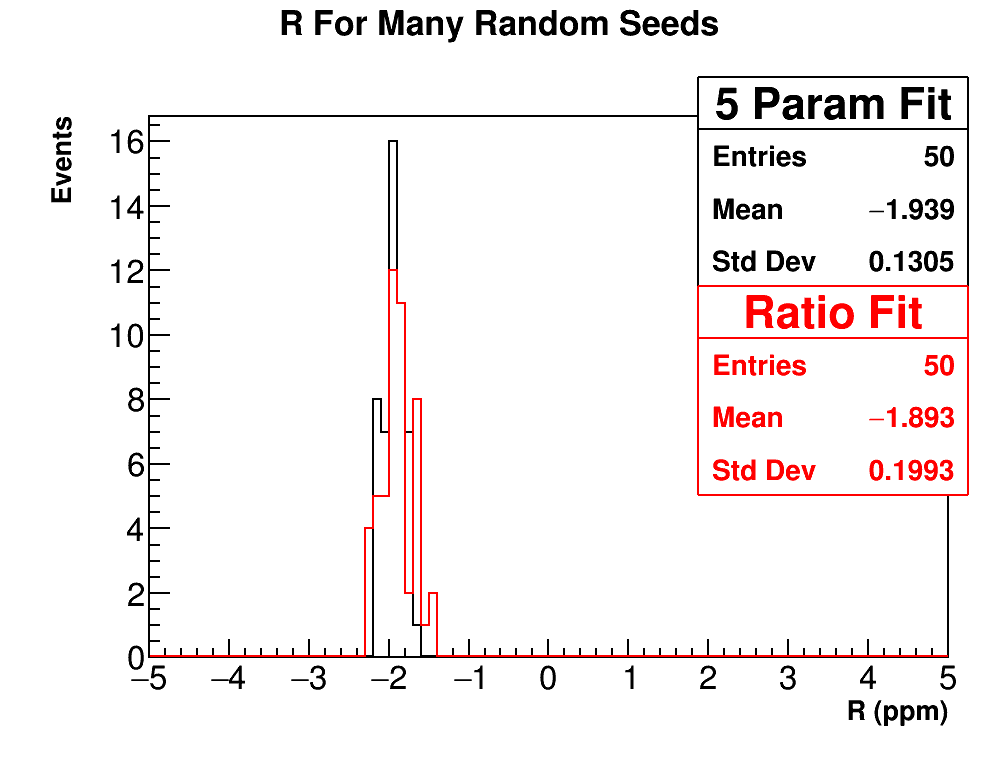
\includegraphics[width=\textwidth]{singleDist_canvas}
		    \caption{Fitted R distributions for a single pseudo-experiment for 5 parameter and 3 parameter ratio fits, for 50 different random seeds.}
		\label{Subfig:SingleRDist}
	    \end{subfigure}
	   	\hspace{4mm}
	    \begin{subfigure}[t]{0.45\textwidth}
		    \centering
			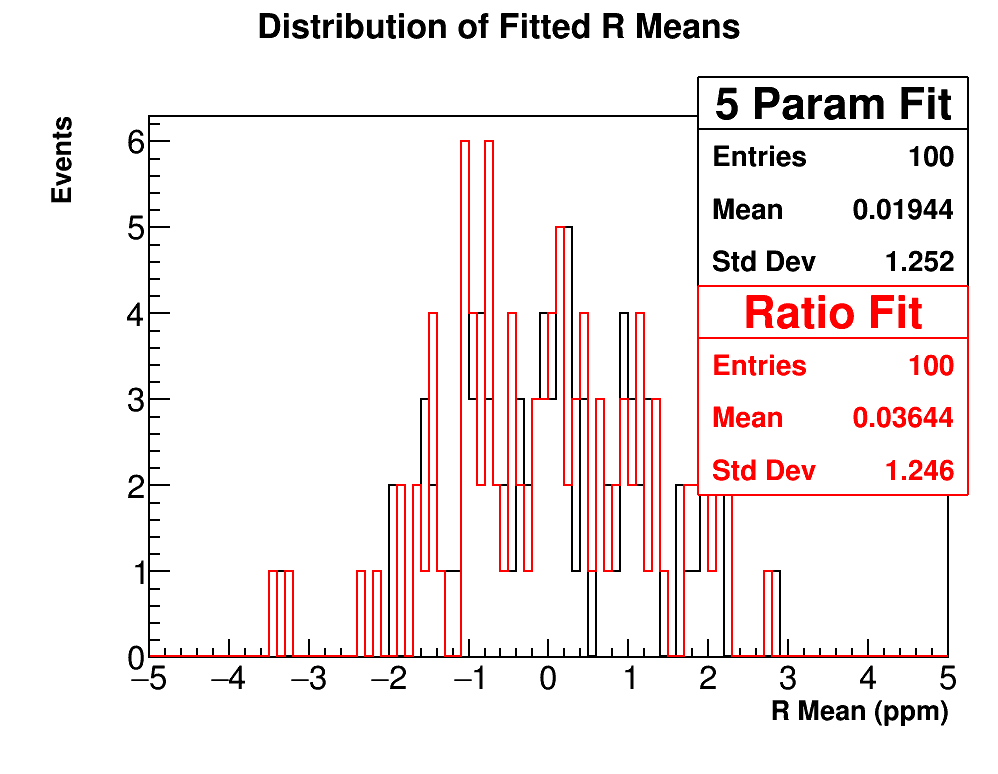
\includegraphics[width=\textwidth]{mean_canvas}
		    \caption{The distribution of means of the fitted R distributions, for 100 separate pseudo-experiments.}
		\label{Subfig:MeanDist}
	    \end{subfigure}% %you need this % here to add spacing between subfigures
	    \vspace{4mm}
	    \begin{subfigure}[t]{0.45\textwidth}
		    \centering
			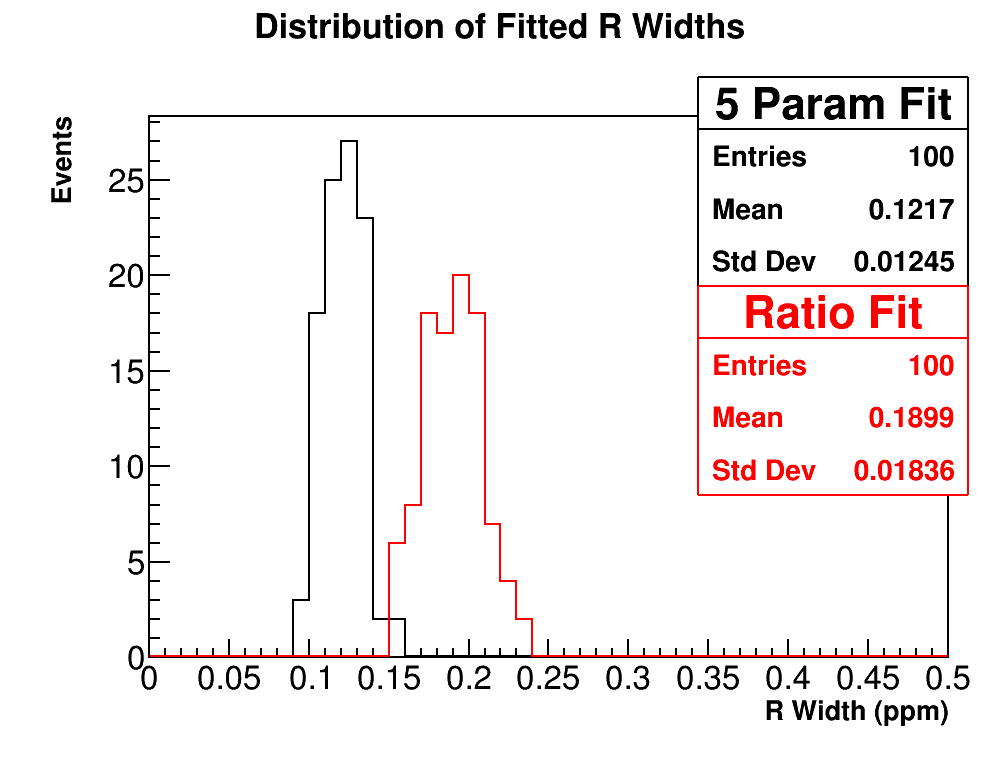
\includegraphics[width=\textwidth]{width_canvas}
		    \caption{The distribution of widths of the fitted R distributions, for 100 separate pseudo-experiments.}
		\label{Subfig:WidthDist}
	    \end{subfigure}
	   	\hspace{4mm}
	    \begin{subfigure}[t]{0.45\textwidth}
		    \centering
			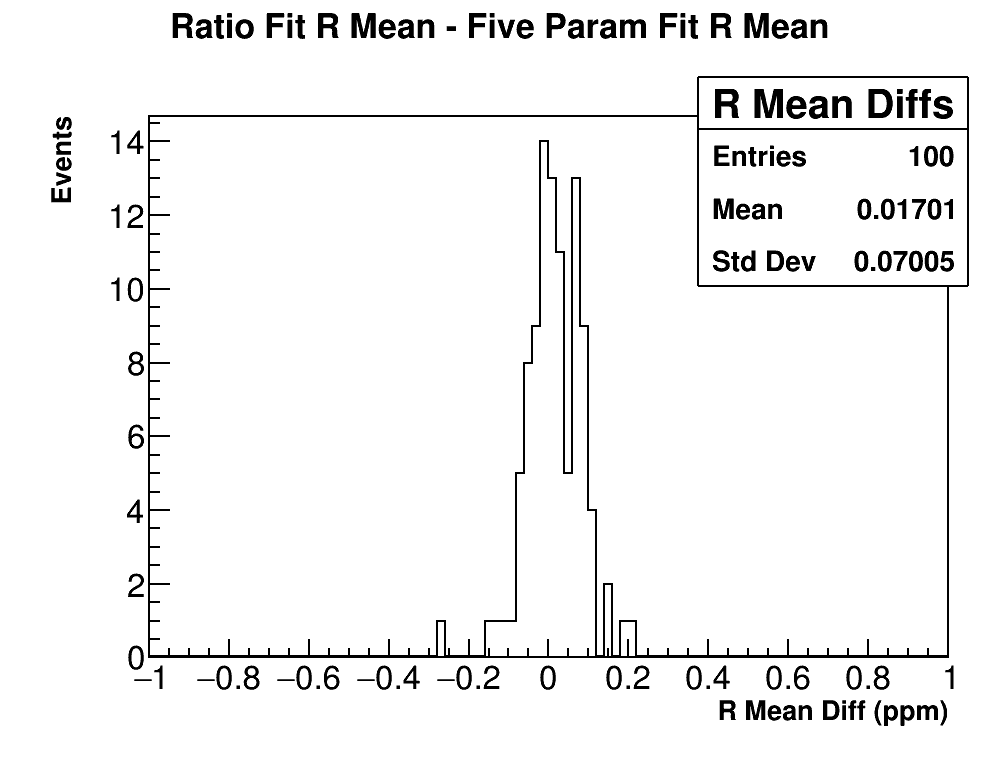
\includegraphics[width=\textwidth]{diff_canvas}
		    \caption{The distribution of differences in fitted R means between 5 parameter fits and 3 parameter ratio fits per pseudo-experiment for 100 pseudo-experiments.}
		\label{Subfig:DiffDist}
	    \end{subfigure}% %you need this % here to add spacing between subfigures
	\caption[TMethodComparison]{MC comparison between T method and ratio method fits for various sets of generated hits and many random seeds. The statistical precision on R for a single fit is approximately 1.3 ppm.}
	\label{fig:TMethodComparison}
	\end{figure}


